%===================================== CHAP 7 =================================

\chapter{Project Life Cycle}

\section{Planning and Research}
The group initiated the project with a planning and research phase, lasting from January the 11th to February the 3rd. 

\subsection{Planning}
The importance of the planning phase was emphasised by the group to avoid being forced to start over because the project was insufficient according to what the customer wanted. \\

The planning phase was initiated by thoroughly choosing the right project, focusing on the strengths and weaknesses within the group. To ensure that every member had the same ambitions and a common understating of what the group expected of each other, a group contract was also formulated. This contract has been important for the group dynamic (see appendix \ref{group_contract}). The risk analysis (see \ref{riskAnalysis}) was also developed during the planning phase, as issues might arise unexpectedly and needed to be managed in a proper fashion. The risk analysis was used to prevent and mitigate issues as they were to happen.  \\  

As the project was assigned - the group prioritized to establish contact with the customer to get a more precise idea of what was to be developed. A contract between the team and the customer was also formulated - ensuring both parties held the same expectations for the project, and of each other during the development process (see appendix \ref{customer_contract}).\\

As the group achieved a better idea of what the project implied - a set of roles were created. These were delegated to the group members depending on prior experience and wishes (see \ref{projectOrganisation}).

\subsection{Research}
In advance of starting the development of the project a thorough research were completed.

Initially the group researched what type of methodology would suit the project, the customer and the group it self (see \ref{methodology}). As the methodology was chosen the group researched what tools facilitated an effortless use of this. The group members have a lot experience in using different tools, which opened for many opportunities for deciding what should be used (see \ref{tools}).

One of the requirements from the customer was a web portal applying the principles of universal design (see \ref{universalDesign}). This is an aspect few of the group members had experience with. Taking this into account the customer provided a resource, DIFI - Universal design principles \cite{Difi}. During the development process, design choices, such as focus marking and colours, has been influenced on knowledge acquired utilising this resource. 

The customer provided several alternative solutions (see \ref{alternativeSolutions}) for the group to explore.  This was primarily done to see how to best satisfy the users' needs. To give the group the best possible understanding of the users' needs there was arranged a workshop together with the users and the providers (see \ref{workshop}). 


\subsubsection{Workshop With Users and Providers}
\label{workshop}
During the researching phase two of the group members, Andresen and Skaugvoll, attended a workshop to map the requirements the users had to the web-portal. 

The workshop was divided into two parts; one with the providers of the activities which are to be posted on the site, and one with the children and parents which would use the site to find the respective activities. The workshop revealed the different needs the users had to the web-portal; especially emphasizing how these differed based on user type, but all functionality should be accessible from the same portal. 

Based on the knowledge Andresen and Skaugvoll acquired throughout the workshop the group got a more definite idea of what should be developed. See appendix \ref{workshop_one} for a summary of the workshop.

\begin{figure}[h!]
\centering
    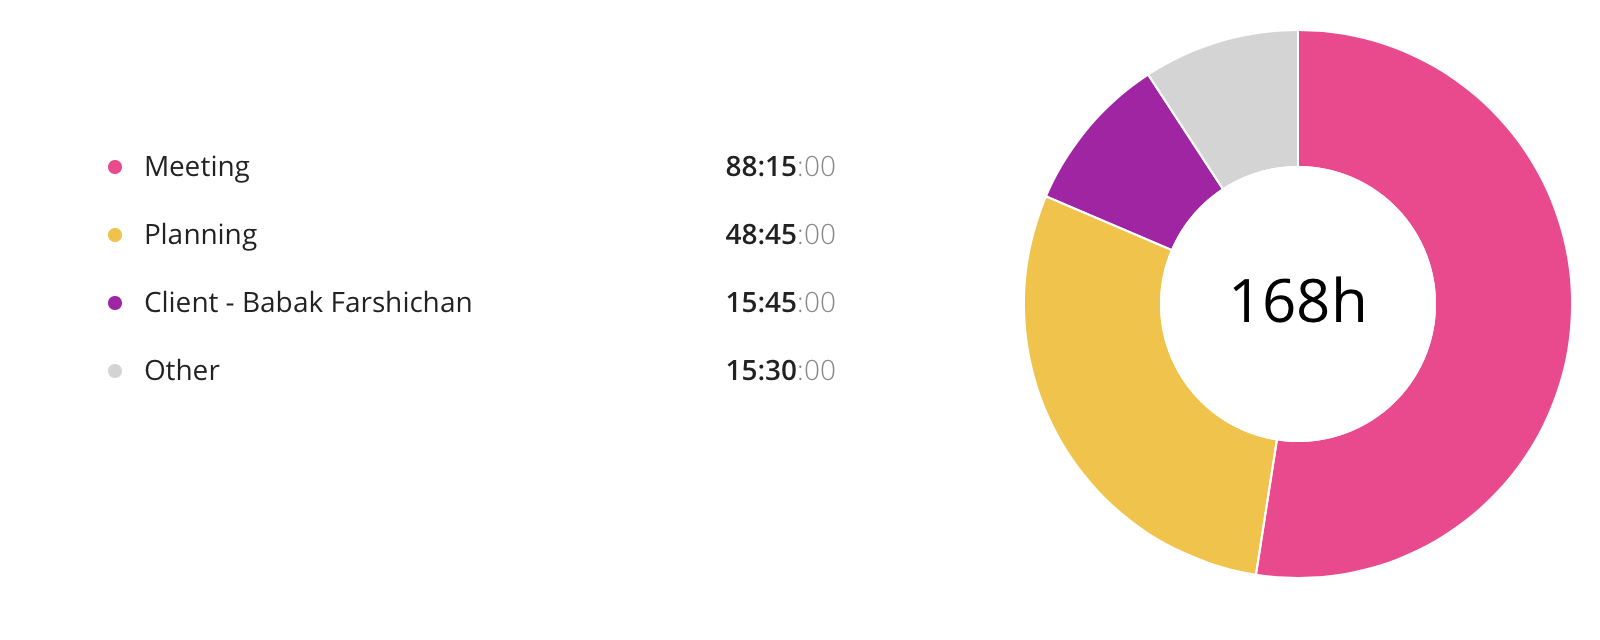
\includegraphics[width=0.4\textwidth]{fig/planning-and-research-diagram}
\caption{Planning and research, hours distributed to work tasks}
\end{figure}


\section{Sprint 0}
\label{sprint0}
The sprint goal for sprint 0 was "Create first design draft, planning and set up product backlog."

Sprint 0 did not have any user stories. Instead the sprint was used to set up the workspace, create an index template in Django, create a product backlog with the customer, decide the MVP (see \ref{MVP}), create a first design draft of the application and doing as much planning as possible. The group chose to do it this way, so the development could start already in the beginning of sprint 1.

The design draft was drawn as a paper prototype, and the group performed a demonstration to the customer. He was satisfied with the idea, and it created a great discussion about how the group should continue working.

\subsubsection{Sprint retrospective meeting summary}
The group are satisfied with their own efforts. Heaps of work are accomplished, and everyone are motivated to keep working next week.
    
The group agrees that they should be more effective in their work sessions, so they can accomplish more. To do this it is important that everyone take responsibility of keeping the group on track, and tell if people are not concentrate on the task.

\begin{figure}[h!]
\centering
    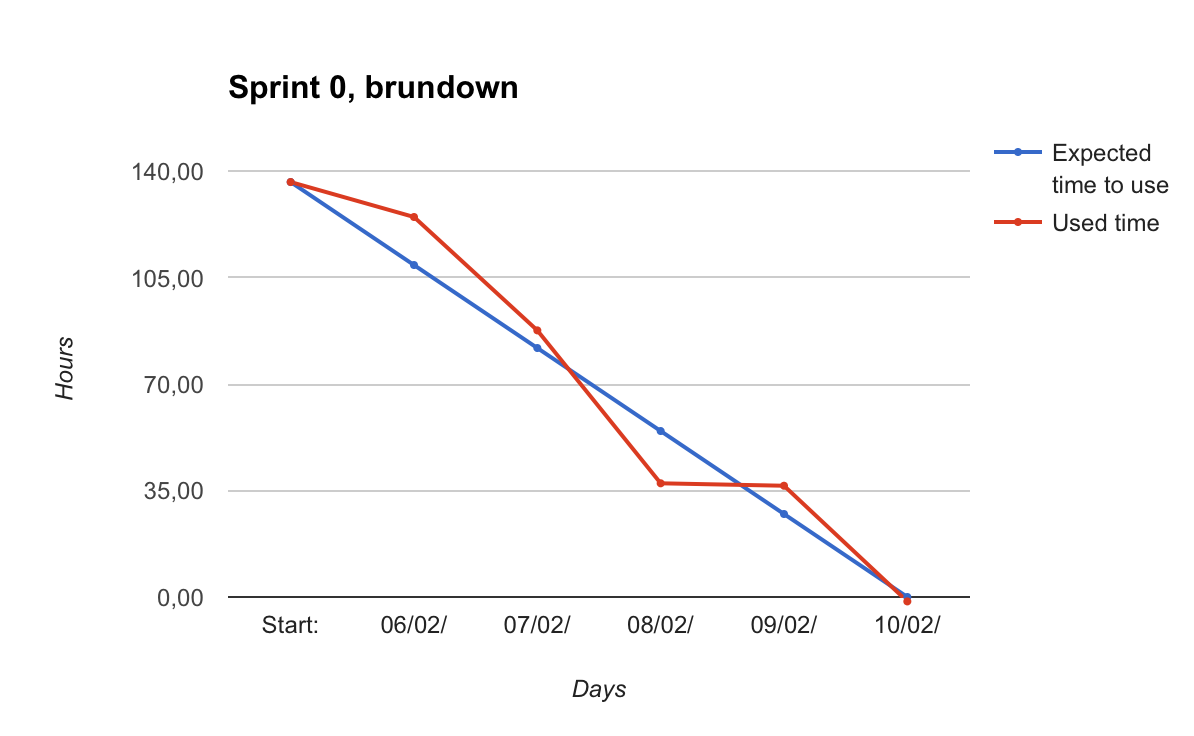
\includegraphics[width=0.8\textwidth]{fig/sprint0}
\caption{Sprint 0, burndown}
\end{figure}

\begin{figure}[h!]
\centering
    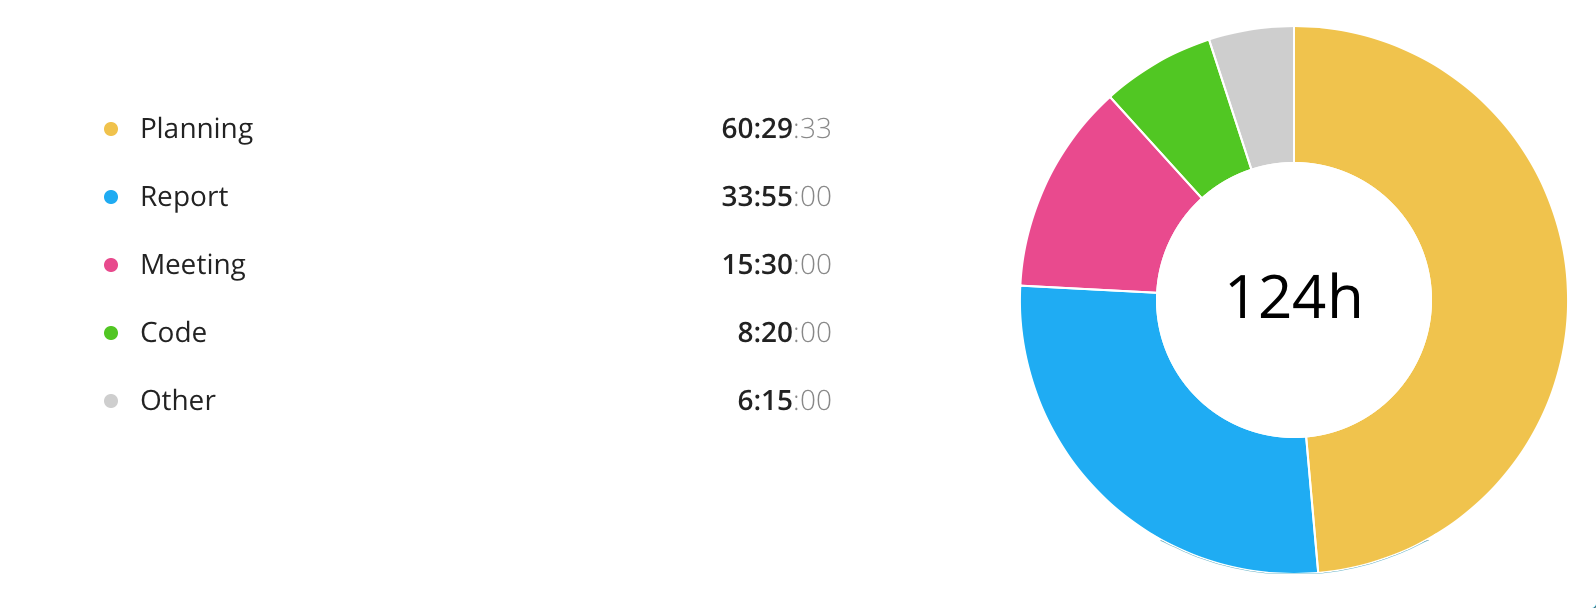
\includegraphics[width=0.8\textwidth]{fig/sprint0-diagram}
\caption{Sprint 0, hours distributed to work tasks}
\end{figure}



\section{Sprint 1}
The overall sprint goal for sprint 1 was to "Deliver first interactive prototype to customer". To achieve this goal, the group created milestones during the sprint planning, that should be finalized during the iteration. The milestones were as as follows: 
\begin{itemize}
  \item Create a mock up database.
  \item Create a flow diagram.
  \item Create issues on GitHub.
  \item Make log in, with different GUI for each role (child, parent, activity      provider, maintainer and anonymous).
  \item Log in with Facebook.
  \item Anonymous user should maybe not be able to see who is going to a activity anonymous should not be able to sign up for activity, before the user has logged in.
  \item  Site map Create skeleton for all pages in site map Investigate the possibility of changing the language (create a dynamic page where all words are listed)
  \item Update wiki (to have the flow diagram, site map and user manual)
\end{itemize}
 
There was two problems encountered this sprint. The first one was that one group member asked for five days of to travel. The group concluded that it was to much to do the upcoming week, and could not give permission for that member to leave. To handle such problems in the future, the group updated their risk analysis. 

The second problem encountered was a misunderstanding between the group and the customer. The group thought that the web portal should be ready to deliver at the end of the project, but the customer only wanted a "Proof of Concept" project. We resolved this with a new meeting with customer and a technical manager at Sintef Digital, and discussed what the groups possibilities were. The problem was solved during that meeting, and the group also updated their risk analysis.

Because of the misunderstanding with the customer, the group had a discussion on how much time to actually spend on the project. After resolving the misunderstanding with customer, the group concluded that the already scheduled hours should remain.


\begin{figure}[h!]
\centering
    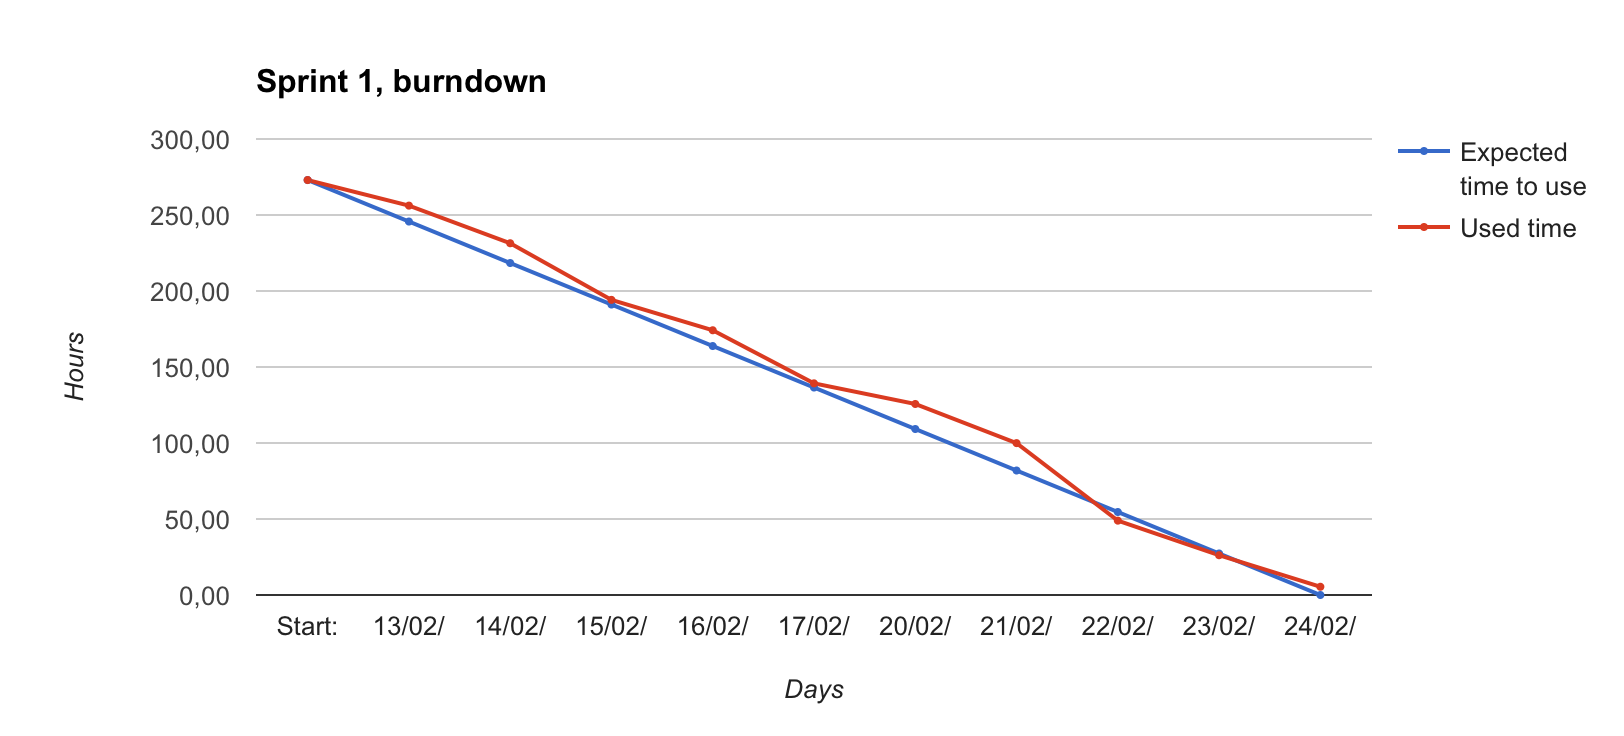
\includegraphics[width=0.8\textwidth]{fig/sprint1}
\caption{Sprint 1, burndown}
\end{figure}

\begin{figure}[h!]
\centering
    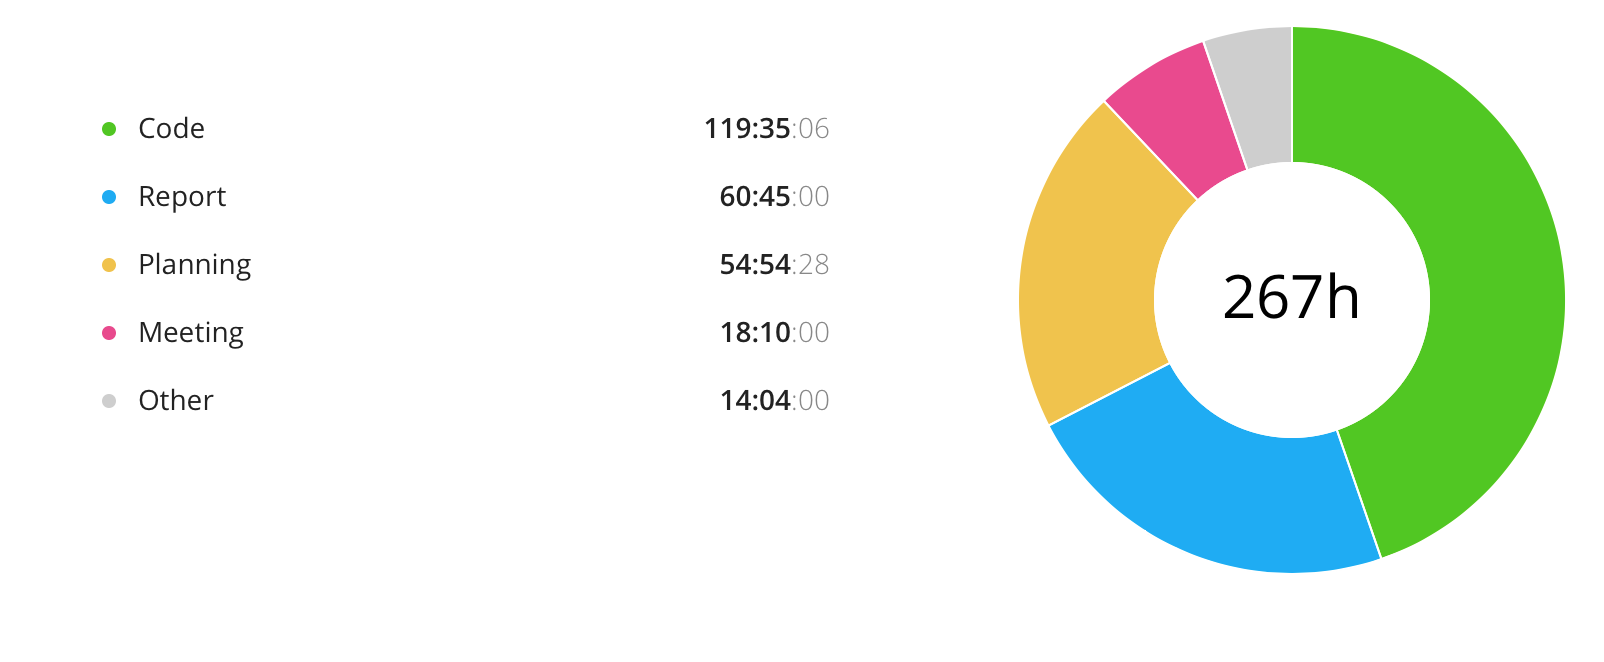
\includegraphics[width=0.8\textwidth]{fig/sprint1-diagram}
\caption{Sprint 1, hours distributed to work tasks}
\end{figure}


\subsubsection{Webserver vs. Webhotel}
The platform for the web portal stood between Webhotel or VPS - virtual private server.  The group had several meetings with the customer regarding this decision. The customer primarily wanted to use web hotel as hosting service and platform. The group proposed to use VPS because it gave a lot of benefits and not constraints like using web hotel would give. 

The group presented to use VPS because it allows for developing the graphical user interface faster and easier by allowing usage of library and frameworks, that webhotels doesn't.  Thus time and resources would be more efficiently allocated. Security is also higher with the use of VPS because it doesn't use a shared resource. If the web portal was hosted through a web hotel, the security of the page and its information would only be protect as much as the less secure webpage that also uses the same shared resource. Hosting on VPS would provide more security for the users of the web portal, and since the product potentially holds sensitive information about the users, security is not to be taken for granted.  Experience also played a part in the decision. The group has more experience with the usage of VPS compared to web hotels. 

Regarding functionality and the project requirements, the platform could be either one, but the usage of VPS would give a much easier development and allow usage of the best suitable technology for the given task. 

The group presented the customer with the proposal to use VPS instead of webhotel, and was engaged in a consulting meeting with the customer, outside developer and the group. The group emphasized that the usage of VPS was just a suggestion, and that it was up to the customer to choose. The project could be done with both.  

\section{Sprint 2}
The goal for sprint 2 was to implement functionality on the activities page; allowing the user to create and retrieve events, as well as filter these. The milestones in sprint 2 were as follows:

\begin{itemize}
  \item Fill database.
  \item Create events.
  \item Retrieve events.
  \item Filter events.
  \item Log in.
  \item Sign up for event.
\end{itemize}

The group met upon a couple of problems during this sprint. Firstly, the group came across problems trying to implement the possibility to filter the activities. Initially the group had chosen to use flux to manage the data flow in the application. With further research and attempts trying to implement the flux pattern the group realised it would not be sufficient in this project, as the application was required to support asynchronous actions. To solve this issue the group was required to complete further research on how this should be implemented, which consumed more of the sprint than first expected. Midway in the sprint the group decided to use Redux (see \ref{redux}) and further research had to be completed on how this is implemented. Due to these issues the milestone, filter events, had to be relocated to sprint 3. 

Another coincidence the group had to manage during sprint 2 was the costumer re-prioritized what was desired to be completed. During sprint 1 a set of milestones was defined and arranged after priority which the group used to define the sprint backlogs. Midway in sprint 2 the customer arouse the desire for one of the final milestones, first version of release up and running on server, to be completed. To fulfill the customer's desire the group highly prioritized this milestone, which induced difficulties completing the original issues in the sprint backlog. To encounter this issue the group decided to re-prioritise the backlog subsequently after the requests from the customer, moving the milestone at hand to sprint 2 and relocate the milestone "Sign up for activity" to sprint 3. 

Even tough the group encountered a couple of problems which affected what was included in the sprint backlog, and subsequently the sprint goal, the group was happy with what they managed to accomplish. A lot of functionality was implemented and the group have been working very well during this period. To improve to later sprints the group should focus issues in the sprint backlog, and not start developing functionality from the product backlog before the issues at hand are completed. 

\begin{figure}[h!]
\centering
    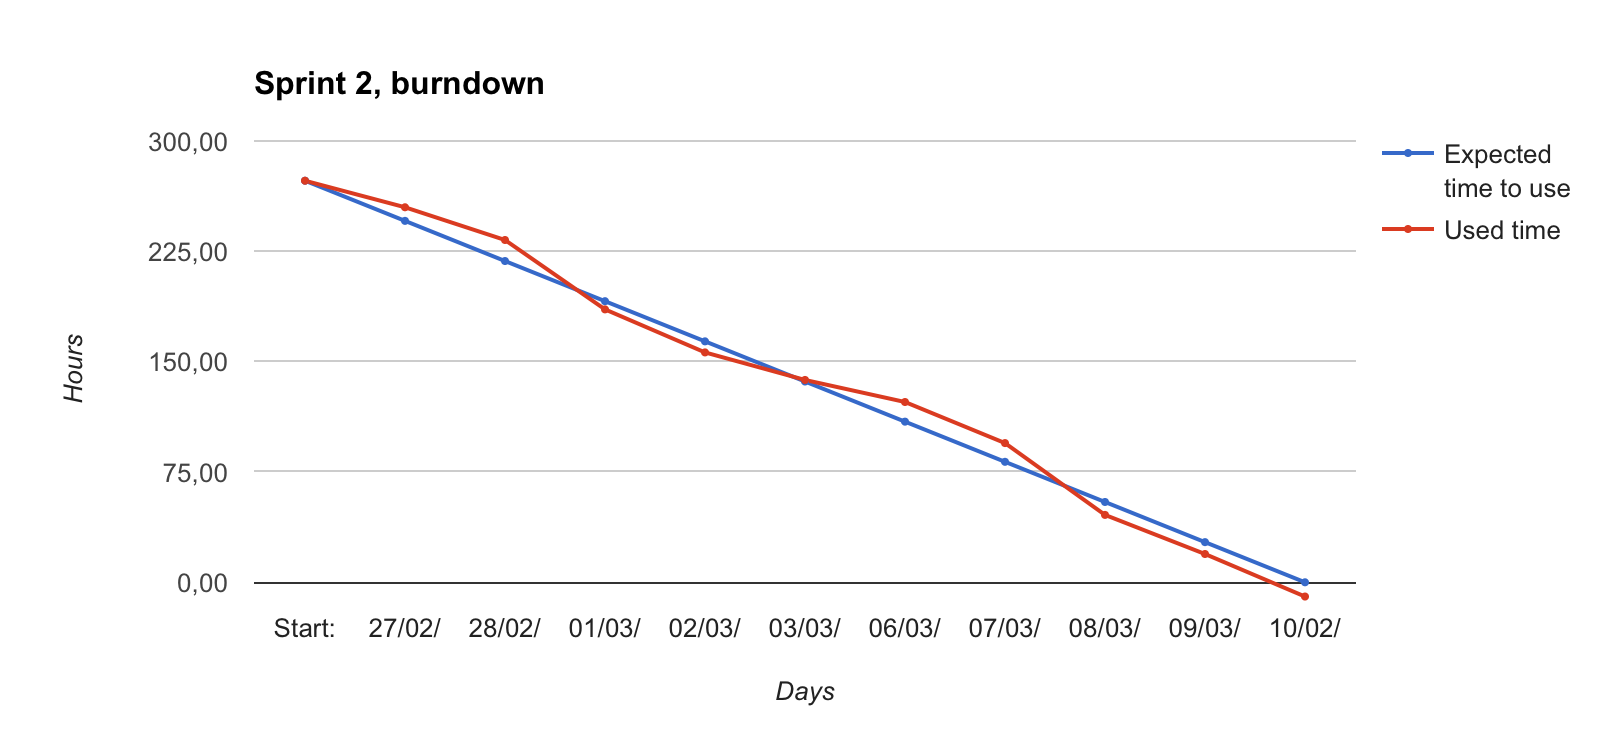
\includegraphics[width=0.8\textwidth]{fig/sprint2}
\caption{Sprint 2, burndown}
\end{figure}

\begin{figure}[h!]
\centering
    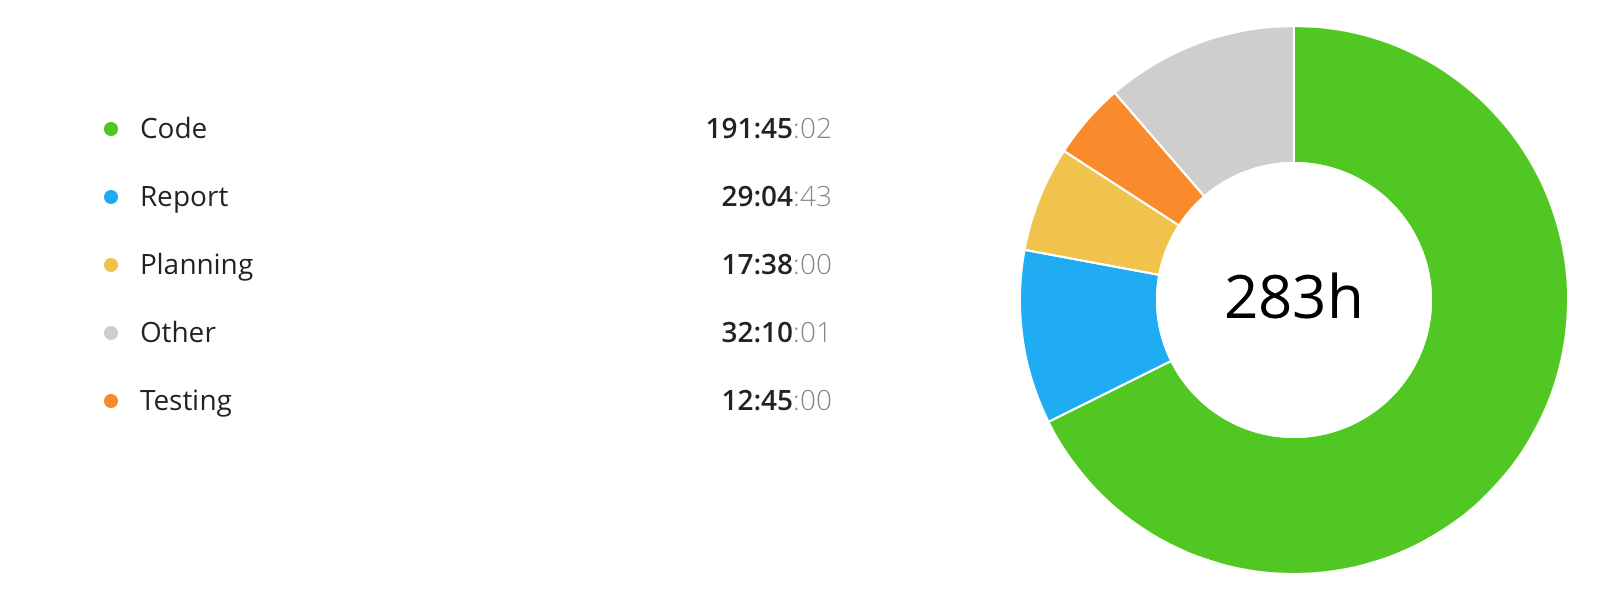
\includegraphics[width=0.8\textwidth]{fig/sprint2-diagram}
\caption{Sprint 2, hours distributed to work tasks}
\end{figure}

\section{Sprint 3}
Sprint backlog, burndowncharts, sprint review

\section{Sprint 4}
Sprint backlog, burndowncharts, sprint review

\section{Sprint 5}
Sprint backlog, burndowncharts, sprint review

\cleardoublepage